\section{Evaluation}
\label{sec:parikshanEvaluation}

To evaluate the performance of \parikshan, we pose and answer the following research questions:

\begin{itemize}
\item \textbf{RQ1:} How long does it take to create a live clone of a production container and what is it's impact on the performance of the production container?
\item \textbf{RQ2:} What is the size of the debugging window, and how does it depend on resource constraints? 
%\item \textbf{RQ3:} Can we generalize the results of our case study to see if \parikshan can target even more real bugs?
\item \textbf{RQ3:} What is the performance overhead of our network duplicator on a service oriented applications? In particular how does forwarding packets to the debugger impact latency, bandwidth and throughput of the application? Does slowdown in debug container impact production service? 
\end{itemize}

We evaluated the \textbf{internal mode} on two identical VM's with an Intel i7 CPU, with 4 Cores, and 16GB RAM each in the same physical host (one each for production and debug containers).
We evaluated the \textbf{external mode} on two identical host nodes with Intel Core 2 Duo Processor, 8GB of RAM.
All evaluations were performed on CentOS 6.5.

%In Section~\ref{sec:performance}, we evaluate live cloning on real-world applications and workloads as well as a micro-benchmark to understand its performance in different scenarios.
%In Section~\ref{sec:timewindowPerformance}, we first provide debug-window sizes for varying workloads run on a live production system. 
%For a more systematic understanding of the debug-window size, we also provide simulation results to show the relationship of buffer overflow with buffer size, the incoming workload, and the instrumentation overhead.
%Finally, in Section~\ref{sec:survey}, we present a survey of 217 real-world bugs, picked from three different applications.
%\xxx{What is the environment we evaluated in? Hardware? Software? Why do we have both real and simulated data?}

\subsection{Live Cloning Performance}
\label{sec:parikshanPerformance}

As explained in Section \ref{sec:parikshanDesign}, a short suspend time during live cloning is necessary to ensure that both containers are in the exact same system state.
The suspend time during live cloning can be divided in 4 parts: 
(1) Suspend \& Dump: time taken to pause and dump the container, 
(2) Pcopy after suspend: time required to complete rsync operation 
(3) Copy Dump File: time taken to copy an initial dump file.
(4) Undump \& Resume: time taken to resume the containers. 
To evaluate ``live cloning'', we ran a micro-benchmark of I/O operations, and evaluated live-cloning on some real-world applications running real-workloads.

\begin{figure}[ht]
	\centering
	\resizebox{.8\linewidth}{!}{
		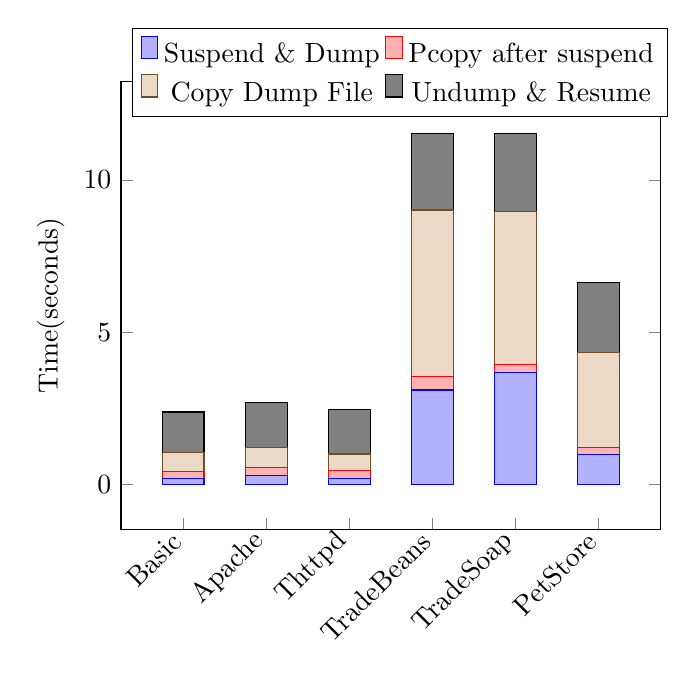
\begin{tikzpicture}
		\begin{axis}[
		ybar stacked,
		bar width=15pt,
		%	nodes near coords,
		enlargelimits=0.15,
		legend style={at={(0.02,1.12)},anchor=north west,legend columns=2},
		ylabel={Time(seconds)},
		symbolic x coords={Basic, Apache, Thttpd, TradeBeans, TradeSoap, 
			PetStore},
		xtick=data,
		x tick label style={rotate=45,anchor=east},
		]
		\addplot+[ybar] plot coordinates {(Basic,0.21) (Apache,0.30) (Thttpd,0.21) (TradeBeans,3.10) (TradeSoap,3.68) (PetStore,0.97) };
		\addplot+[ybar] plot coordinates {(Basic,0.22) (Apache,0.27) (Thttpd,0.26) (TradeBeans,0.44) (TradeSoap,0.25) (PetStore,0.24) };
		\addplot+[ybar] plot coordinates {(Basic,0.62) (Apache,0.64) (Thttpd,0.53) (TradeBeans,5.47) (TradeSoap,5.03) (PetStore,3.11) };
		\addplot+[ybar] plot coordinates {(Basic,1.33) (Apache,1.47) (Thttpd,1.46) (TradeBeans,2.51) (TradeSoap,2.57) (PetStore,2.32) };
		\addlegendentry{\strut Suspend \& Dump}
		\addlegendentry{\strut Pcopy after suspend}
		\addlegendentry{\strut Copy Dump File}
		\addlegendentry{\strut Undump \& Resume}
		\end{axis}
		\end{tikzpicture}
	}
	%\captionsetup{justification=centering}
	\caption{Suspend time for live cloning, when running a representative benchmark}
	\label{fig:stats}
\end{figure}


\subsubsection{Real world applications and workloads:}
To begin to study the overhead of live cloning, we performed an evaluation using five well-known applications.
Figure~\ref{fig:stats} presents the suspended times for five well-known applications when cloning a replica with \parikshan. 
We ran the httperf~\cite{httperf} benchmark on Apache and \emph{thttpd} to compute max throughput of the web-servers, by sending a large number of concurrent requests.
Tradebeans and Tradesoap are both part of the dacapo~\cite{dacapo} benchmark ``DayTrader'' application.
These are realistic workloads, which run on a multi-tier trading application provided by IBM. 
PetStore~\cite{petstore} is also a well known J2EE reference application. 
We deployed PetStore in a 3-tier system with JBoss, MySQL and Apache servers, and cloned the app-server.
The input workload was a random set of transactions which were repeated for the duration of the cloning process.

As shown in Figure~\ref{fig:stats}, for Apache and Thttpd the container suspend time ranged between 2-3 seconds.
However, in more memory intensive application servers such as PetStore and DayTrader, the total suspend time was higher (6-12 seconds).
Nevertheless, we did not experience any timeouts or errors for the requests in the workload\footnote{In case of packet drops, requests are resent both at the TCP layer, and the application layer. This slows down the requests for the user, but does not drop them}.
However, this did slowdown requests in the workload. 
This shows that short suspend times are largely not visible or have minimal performance impact to the user, as they are within the time out range of most applications.
Further, a clean network migration process ensures that connections are not dropped, and are executed successfully.
We felt that these relatively fast temporary app suspensions were a reasonable price to pay to launch an otherwise overhead-free debug replica.
To further characterize the suspend time imposed by the live cloning phase of \parikshan, we created a synthetic micro-benchmark to push \parikshan towards its limit.
\begin{figure}[ht]
	%{0.45\textwidth}
	\centering
	\resizebox{.8\linewidth}{!}{
		%\begin{adjustbox}{max size={.9\textwidth}}
		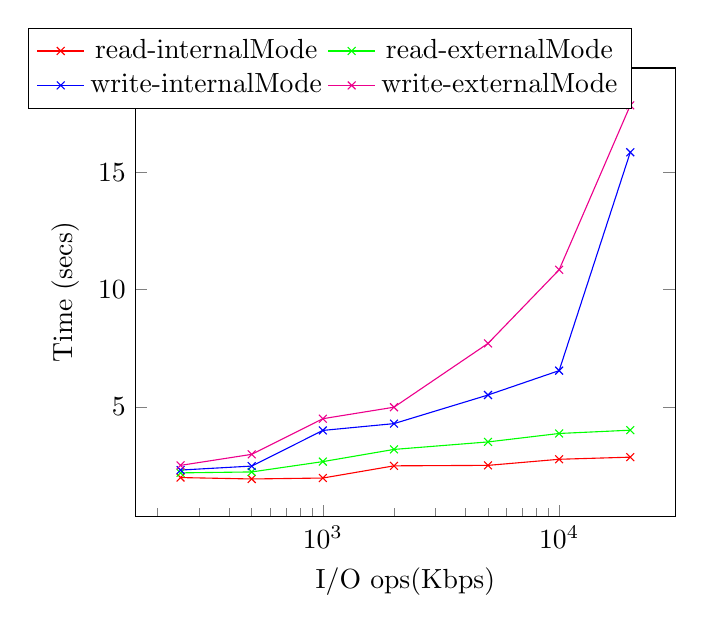
\begin{tikzpicture}
		\begin{axis}[
		xmode=log,
		legend style={at={(-0.2,1.09)},anchor=north west,legend columns=2},
		xlabel=I/O ops(Kbps),
		ylabel=Time (secs)]
		\addplot[color=red,mark=x] coordinates {
			(0,1.85)
			(250,1.99)
			(500,1.93)
			(1000,1.97)
			(2000,2.49)
			(5000,2.51)
			(10000,2.77)
			(20000,2.86)
		};
		\addlegendentry{read-internalMode}
		\addplot[color=green,mark=x] coordinates {
			(0,1.97)
			(250,2.19)
			(500,2.23)
			(1000,2.67)
			(2000,3.19)
			(5000,3.51)
			(10000,3.87)
			(20000,4.01)
		};
		\addlegendentry{read-externalMode}				
		\addplot[color=blue,mark=x] coordinates {
			(0,1.85)
			(250,2.31)
			(500,2.48)
			(1000,4.00)
			(2000,4.29)
			(5000,5.51)
			(10000,6.55)
			(20000,15.86)
		};
		\addlegendentry{write-internalMode}				
		\addplot[color=magenta,mark=x] coordinates {
			(0,1.87)
			(250,2.51)
			(500,2.98)
			(1000,4.50)
			(2000,4.99)
			(5000,7.71)
			(10000,10.85)
			(20000,17.86)
		};
		\addlegendentry{write-externalMode}
		\end{axis}
		\end{tikzpicture}
		% \end{adjustbox}
	}
	%\captionsetup{justification=centering}
	\caption{Live Cloning suspend time with increasing amounts of I/O operations }
	\label{fig:fioResults}
\end{figure}



\subsubsection{Micro Benchmark using I/O operations:}
The main factor that impacts suspend time is the number of ``dirty pages'' in the suspend phase, which have not been copied over in the pre-copy rsync operation (see section~\ref{sec:parikshanCloneManager}).
To understand this better, we use \fio (flexible I/O tool for Linux)~\cite{fio}, to gradually increase the number of I/O operations while doing live cloning.
We run the \fio tool to do read and writes of random values with a controlled I/O bandwidth. 
%The suspend time is observed by instrumentation within the cloning script, which reports time taken by each of the suspend processes.
Additionally, we ensure that the I/O job being processed by \fio is long enough to last through the cloning process.

As shown in figure~\ref{fig:fioResults}, read operations have a much smaller impact on suspend time of live cloning compared to write operations.
This can be attributed to the increase of ``dirty pages'' in write operations, whereas for read, the disk image remains largely the same.
The internal mode is much faster than the external mode, as both the production and debug-container are hosted in the same physical device.
We believe, that for higher I/O operations, with a large amount of ``dirty-pages'', network bandwidth becomes a bottleneck: leading to longer suspend times.
Overall in our experiments, the internal mode is able to manage write operation up to 10 Mbps, with a total suspend-time of approx 5 seconds.
Whereas, the external mode is only able to manage up to 5-6 Mbps, for a 5 sec suspend time.\\ \\

\begin{tcolorbox}[breakable, enhanced]
	To answer \textbf{RQ1}, live cloning introduces a short suspend time in the production container dependent on the workload. 
	Write intensive workloads will lead to longer suspend times, while read intensive workloads will take much less. 
	Suspend times in real workload on real-world systems vary from 2-3 seconds for webserver workloads to 10-11 seconds for application/database server workloads. 
	Compared to external mode, internal mode had a shorter suspend time. 
	A production-quality implementation could reduce suspend time further by rate-limiting incoming requests in the proxy, or using copy-on-write mechanisms and faster shared file system/storage devices already available in several existing live migration solutions.
\end{tcolorbox}

\subsection{Debug Window Size}
\label{sec:parikshanTimewindowPerformance}

To understand the size of the debug-window and it's dependence on resources, we did some experiments on real-world applications, by introducing a delay while duplicating the network input.
This gave us some real-world idea of buffer overflow and it's relationship to the buffer size and input workload.
Since it was difficult to observe systematic behavior in a live system to understand the decay rate of the debug-window, we also did some simulation experiments, to see how soon the buffer would overflow for different input criteria.

\xxx{We did some experiments, and also simulations because... The setup was... The buffer size was...}
\yyy{added the reason, as a small intro}

\begin{table}[ht]
	\centering
	\setlength{\tabcolsep}{2pt}
	\begin{tabular}{c c c c }
		\toprule
		{\bf Input Rate} & \textbf{Debug Window} & \textbf{Pipe Size} & \textbf{Slowdown} \\ \midrule
		530 bps, 27 rq/s & $\infinity$ & 4096 & 1.8x \\ %\hline
		530 bps, 27 rq/s & 8 sec & 4096 & 3x \\ %\hline
		530 bps, 27 rq/s & 72 sec & 16384 & 3x \\ %\hline
		Pois., $\lambda$ = 17 rq/s & 16 sec & 4096 & 8x \\ %\hline
		Pois., $\lambda$ = 17 rq/s & 18 sec & 4096 & 5x \\ %\hline
		Pois.,$\lambda$ = 17 rq/s & $\infinity$ & 65536 & 3.2x \\ %\hline
		Pois.,$\lambda$ = 17 rq/s & 376 sec & 16384 & 3.2x \\ %\hline
		\bottomrule
	\end{tabular}
	%\captionsetup{justification=centering}
	\caption{Approximate debug window sizes for a MySQL request workload}
	\label{table:timewindow}
\end{table}

\noindent
\textbf{Experimental Results:} We call the time taken to reach a buffer overflow the ``debug-window''.
As explained earlier, the size of this debug-window depends on the overhead of the ``instrumentation'', the incoming workload distribution, and the size of the buffer.
To evaluate the approximate size of the debug-window, we sent requests to both a production and debug MySQL container via our network duplicator.
Each workload ran for about 7 minutes (10,000 ``select * from table'' queries), with varying request workloads.
We also profiled the server, and found that is able to process a max of ~30 req/s\footnote{Not the same as bandwidth, ~30 req/s is the maximum rate of sequential requests MySQL server is able to handle for a user session} in a single user connect session. 
For each of our experiments, we vary the buffer sizes to get an idea of debug-window. 
Additionally, we generated a slowdown by first modeling the time taken by MySQL to process requests (27 req/s or 17req/s), and then putting an approximate sleep in the request handler.

Initially, we created a connection and sent requests at 90\% of the maximum request rate the server was able to handle (27 req/s).
We found that for overheads up-to 1.8x (approx) we experienced no buffer overflows.
For higher overheads the debug window rapidly decreased, primarily dependent on buffer-size, request size, and slowdown.

%Next, we mimic user behavior, to generate a realistic workload.
We then sent requests at about 60\% of the maximum request rate i.e. average 17 req/s. 
The requests were sent at varying intervals using a poisson distribution. 
This varies the inter-request arrival time (this is similar to production requests under normal workloads) and let's the cloned debug-container catch up with the production container during idle time-periods in between request bursts.
We observed, that compared to earlier experiments, there was more slack in the system. 
This meant that our system was able to tolerate a much higher overhead (3.2x) with no buffer overflows.

Our experiments showed that idle time between requests can be used by the \debugcontainer to catch up to the production container. 
Most production systems run much below the maximum capacity, this would allow the \debugcontainer to catch up to the \productioncontainer thereby allowing for long debug windows.

\begin{figure}[ht]
	%{0.45\textwidth}
	\centering
	\resizebox{.85\linewidth}{!}{
		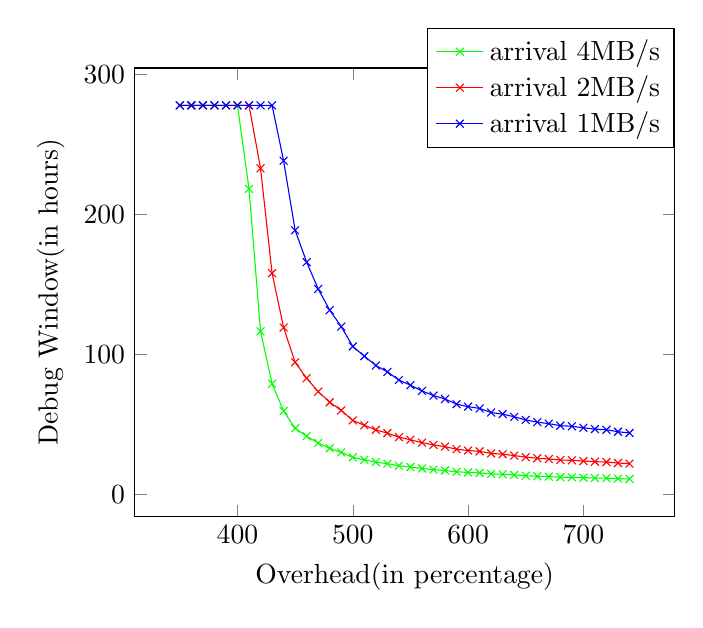
\begin{tikzpicture}
		\begin{axis}[
		%xmode=log,
		legend style={at={(1,1.09)},anchor=north east,legend columns=1},
		xlabel=Overhead(in percentage),
		ylabel=Debug Window(in hours)]
		\addplot[color=green,mark=x] coordinates {
			(350,277.7778028)
			(360,277.7778306)
			(370,277.7777806)
			(380,277.7777806)
			(390,277.777875)
			(400,277.7777972)
			(410,218.0984611)
			(420,116.3991028)
			(430,78.9657)
			(440,59.55381111)
			(450,47.147775)
			(460,41.446375)
			(470,36.65794167)
			(480,32.87560278)
			(490,29.95016111)
			(500,26.40129444)
			(510,24.66028333)
			(520,23.00362222)
			(530,21.85588056)
			(540,20.40405)
			(550,19.48659444)
			(560,18.45943611)
			(570,17.63081111)
			(580,17.01690833)
			(590,16.09901389)
			(600,15.65028056)
			(610,15.33356944)
			(620,14.601075)
			(630,14.32908611)
			(640,13.83495833)
			(650,13.29390556)
			(660,12.88229722)
			(670,12.61861944)
			(680,12.25779722)
			(690,12.14353889)
			(700,11.8762)
			(710,11.64855)
			(720,11.52348611)
			(730,11.17581111)
			(740,10.95483889)
		};
		\addlegendentry{arrival 4MB/s}
		\addplot[color=red,mark=x] coordinates {
			(350,277.7778361)
			(360,277.7777917)
			(370,277.7778389)
			(380,277.7778222)
			(390,277.7777806)
			(400,277.7778056)
			(410,277.7777778)
			(420,232.7982083)
			(430,157.9314)
			(440,119.1076194)
			(450,94.29555)
			(460,82.89275)
			(470,73.31588611)
			(480,65.75120278)
			(490,59.90032222)
			(500,52.80259167)
			(510,49.32056944)
			(520,46.00724722)
			(530,43.71176389)
			(540,40.80809722)
			(550,38.97319167)
			(560,36.91887222)
			(570,35.26162222)
			(580,34.03381667)
			(590,32.19803056)
			(600,31.30056389)
			(610,30.66714167)
			(620,29.20215)
			(630,28.65817222)
			(640,27.66991667)
			(650,26.58781389)
			(660,25.76459444)
			(670,25.23723611)
			(680,24.51559722)
			(690,24.28707778)
			(700,23.75239722)
			(710,23.2971)
			(720,23.046975)
			(730,22.35162222)
			(740,21.909675)
		};
		\addlegendentry{arrival 2MB/s}				
		\addplot[color=blue,mark=x] coordinates {
			(350,277.7778694)
			(360,277.7777944)
			(370,277.7779611)
			(380,277.7778389)
			(390,277.7777889)
			(400,277.7779139)
			(410,277.7778056)
			(420,277.7778167)
			(430,277.777875)
			(440,238.2152389)
			(450,188.5911)
			(460,165.7855028)
			(470,146.6317694)
			(480,131.5024056)
			(490,119.8006444)
			(500,105.6051806)
			(510,98.64113611)
			(520,92.01449444)
			(530,87.42352778)
			(540,81.61619722)
			(550,77.94638056)
			(560,73.83774444)
			(570,70.52324444)
			(580,68.06763333)
			(590,64.39605833)
			(600,62.60112778)
			(610,61.33428056)
			(620,58.40430278)
			(630,57.31634722)
			(640,55.33983056)
			(650,53.175625)
			(660,51.52919167)
			(670,50.474475)
			(680,49.03119167)
			(690,48.57415278)
			(700,47.50479722)
			(710,46.59420278)
			(720,46.09394722)
			(730,44.70324722)
			(740,43.81935)
		};
		\addlegendentry{arrival 1MB/s}				
		\end{axis}
		\end{tikzpicture}
	}
	%\captionsetup{justification=centering}
	\caption{Simulation results for debug-window size. Each series has a constant arrival rate, and the buffer is kept at 64GB.}
	\label{fig:debugSim}
\end{figure}

\noindent
\textbf{Simulation Results:} 
In our next set of experiments, we simulate packet arrival and service processing for a buffered queue in SOA applications. 
We use a discrete event simulation based on an M\/M\/1 queue, which is a  classic queuing model based on Kendall's notation~\cite{kendall}, and is often used to model SOA applications with a single buffer based queue.
Essentially, we are sending and processing requests based on a Poisson distribution with a finite buffer capacity.
In our simulations (see Figure~\ref{fig:debugSim}), we kept a constant buffer size of 64GB, and iteratively increased the overhead of instrumentation, thereby decreasing the service processing time.
Each series (set of experiments), starts with an arrival rate approximately 5 times less than the service processing time. 
This means that at 400\% overhead, the system would be running at full capacity (for stable systems SOA applications generally operate at much less than system capacity).
Each simulation instance was run for 1000000 seconds or 277.7 hours.
We gradually increased the instrumentation by 10\% each time, and observed the \textit{hitting-time} of the buffer (time it takes for the buffer to overflow for the first time).
As shown there is no buffer overflow in any of the simulations until the overhead reaches around 420-470\%, beyond this the debug-window decreases exponentially.
Since beyond 400\% overhead, the system is over-capacity, the queue will start filling up fairly quickly. 
This clarifies the behavior we observed in our experiments, where for lower overheads (1.8-3.2x) we did not observe any overflow, but beyond a certain point, we observed that the buffer would overflow fairly quickly.
Also as shown in the system, since the buffer size is significantly larger than the packet arrival rate, it takes some time for the buffer to overflow (several hours).
We believe that while most systems will run significantly under capacity, large buffer sizes can ensure that our debug-container may be able to handle short bursts in the workload.
However, a system running continuously at capacity is unlikely to tolerate significant instrumentation overhead.\\ \\
%For more details regarding queuing theory models and our detailed simulations, please have a look at our extended tech-report tech-report~\cite{parikshanQueue}.

\xxx{Good to show here a list of example dynamic analyses that would fit within the window. So, say, our GOAL is to be able to support running dynamic analyses X, Y, Z. X, Y, and Z usually have an overhead of 1.5X, which is WAY too slow to use in production. BUT can we use them in our debug environments? YES!}


\begin{tcolorbox}[breakable, enhanced]
	To answer \textbf{RQ2}, we found that the debug-container can stay in a stable state without any buffer overflows as long as the instrumentation does not cause the service times to become less than the request arrival rate. Furthermore, a large buffer will allow handling of short bursts in the workload until the system returns back to a stable state. The debug-window can allow for a significant slowdown, which means that many existing dynamic analysis techniques~\cite{dpor,valgrind}, as well as most fine-grained tracing~\cite{fay,failuresketching} can be applied on the debug-container without leading to an incorrect state.
\end{tcolorbox}



\iffalse
\begin{table}[ht]
	\begin{centering}
		\begin{tabular}{|c|c|c|c|}
			\hline
			\begin{tabular}[c]{@{}c@{}}\textbf{Input} \\ \textbf{Rate}\end{tabular} & \begin{tabular}[c]{@{}c@{}}\textbf{Debug}\\ \textbf{Window}\end{tabular} & \begin{tabular}[c]{@{}c@{}}\textbf{Pipe}\\ \textbf{Size}\end{tabular} & \begin{tabular}[c]{@{}c@{}}\textbf{Slow-}\\ \textbf{down}\end{tabular}\\ \hline
			530 bps, 27 rq/s                                      & $\infinity$                                                    & 4096                                                & 1.8x                      \\ \hline
			530 bps, 27 rq/s                                      & 8 sec                                                  & 4096                                                & 3x                        \\ \hline
			530 bps, 27 rq/s                                      & 72 sec                                                 & 16384                                               & 3x                        \\ \hline
			Poisson, $\lambda$ = 17 rq/s                               & 16 sec                                                 & 4096                                                & 8x                        \\ \hline
			Poisson, $\lambda$ = 17 rq/s                               & 18 sec                                                 & 4096                                                & 5x                      \\ \hline
			Poisson, $\lambda$ = 17 rq/s                               & $\infinity$                                                    & 65536                                               & 3.2x \\ \hline
			Poisson, $\lambda$ = 17 rq/s                               & 376 sec                                                & 16384                                               & 3.2x \\ \hline
		\end{tabular}
		\captionsetup{justification=centering}
		\caption{Approximate debug window sizes for a MySQL request workload}
		\label{table:timewindow}
	\end{centering}
\end{table}
\fi


\subsection{Network Duplication Performance Overhead}
\label{sec:DupPerformanceOverhead}

%TODO- Finish performance overhead
As explained in section~\ref{sec:parikshanOverhead}, a potential overhead in \parikshan is the network level duplication and forwarding. 
For each packet received by the duplicator it is copied to the outgoing buffer of connections to both the production and the debug container. 
The communication to the production and the debug container is done in parallel, using non-blocking I/O. 
This ensures that packet forwarding to the debug-container has a negligible impact on packet-forwarding to production.
Another potential overhead can be because of the extra-hop introduced by a proxy. 
This is easily avoided by coupling our network duplication with existing proxies in the deployed application.
Proxies are commonly used in most SOA applications, for security, and performance purposes~\cite{squid} (they allow caching which gives significant performance boosts).

%While we do have an extra-hop when using the duplication proxy compared to native communication, using proxies is common in most SOA applications, and usually does not incur much overhead.
%TODO cite split tcp effect to improve latency in case of proxy

\begin{comment}
	
\begin{figure}[ht]
	%{0.45\textwidth}
	\centering
	\resizebox{.85\linewidth}{!}{
		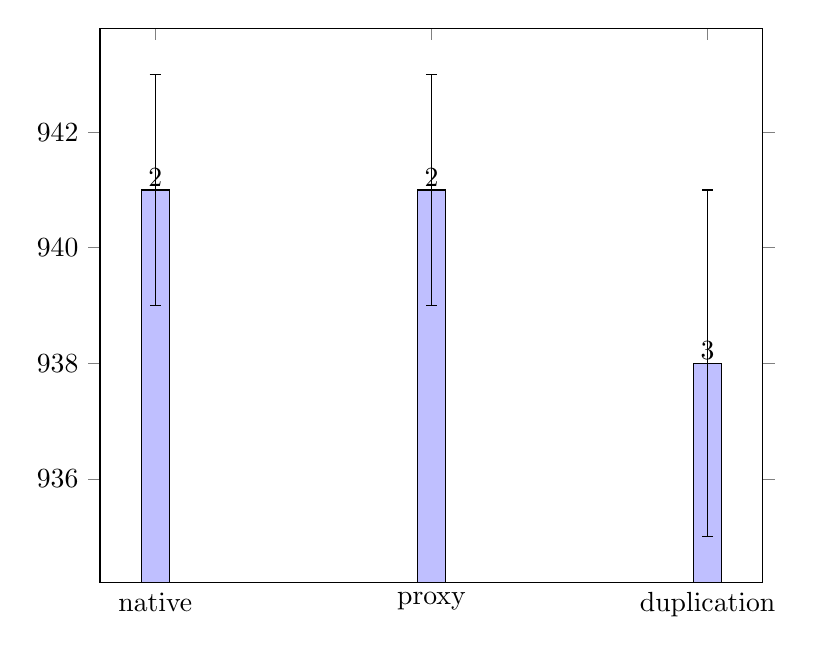
\begin{tikzpicture}
		\begin{axis}[
		%title = {Optimization based upon co-occurences},
		xbar,
		width=10cm,
		xtick={1,2,3},
		xticklabels={%
			native,
			proxy,
			duplication},
		%grid=major,
		]
		
		\addplot[
		fill=blue!25,
		draw=black,
		ybar,
		point meta=y,
		visualization depends on=\thisrow{label} \as \barlabel,
		nodes near coords=\pgfmathprintnumber{\barlabel},
		every node near coord/.style={inner ysep=1pt},
		error bars/.cd,
		y dir=both,
		y explicit
		] 
		table [row sep=crcr, y error=error] {
			x   y           error    label\\
			1   941   2 2 \\
			2   941    2 2 \\
			3   938  3 3 \\
		};
		
		%\draw ({rel axis cs:0,0}|-{axis cs:0,0}) -- ({rel axis cs:1,0}|-{axis cs:0,0});
		\end{axis}
		\end{tikzpicture}
	}
	%\captionsetup{justification=centering}
	\caption{Performance impact on network bandwidth when using network duplication. The above chart shows network bandwidth performance comparison of native execution, with proxy}
	\label{fig:performanceBandwidth}
\end{figure}
\end{comment}

\begin{figure}[!ht]
	\begin{center}
		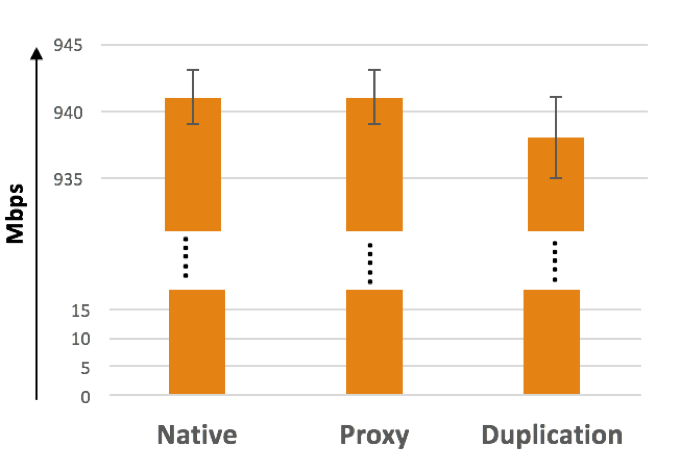
\includegraphics[width=0.7\textwidth]{parikshan/figs/Bandwidth.png}
		\caption{Performance impact on network bandwidth when using network duplication. The above chart shows network bandwidth performance comparison of native execution, with proxy}
		\label{fig:performanceBandwidth}
	\end{center}
\end{figure}

In this section, we have focused on the end-to-end performance overhead of a system running with the debug container and duplicating the network traffic.
For our testing purposes, we have run each of the experiments in the following three modes : 

\begin{itemize}
	\item \textbf{Native:} In this mode we only run the client and the server without any proxy or any external network forwarding. 
	\item \textbf{Proxy Only:} In this mode we have a proxy which is  forwarding packets from the client to the server, without any duplication. 
	\item \textbf{Duplication:} Here we have \parikshan's network duplicator, which is forwarding packets from the client to the server, as well as to the debug container.
\end{itemize}

The server and the proxy run on the same physical machine, in each of the the three modes.
The client, as well as the debug container are run on a different physical machines to avoid resource contention.
Additionally, all components are in the same local subnet.

We divide our evaluation into two parts, first into micro-benchmarks which focus on raw TCP level connection performances, such as impact on bandwidth and latency. Next we look at the impact on two real-world applications - MediaWiki~\cite{mediawiki}, and MySQL~\cite{mysql}.

\subsubsection{Micro-benchmark - Bandwidth and Latency}
\label{sec:microBenchBandwidthLatency}

In order to understand the overhead that our duplicator can have on network performance, we look at how much the network forwarding of TCP packets is impacted by duplication in the proxy. 
This can be in two different aspects, firstly throughput (or bandwidth), and secondly latency.\\


\noindent\textbf{Network Bandwidth:}
To understand the impact of network duplication on the bandwidth between a client and a server we run a micro-benchmark using iperf~\cite{iperf} - a well known tool for performing network throughput measurements. It can test either TCP or UDP communication throughput measurements. 
To perform an iperf test  the  user must establish both a server (to discard traffic) and a client (to generate traffic).

 Figure~\ref{fig:performanceBandwidth} shows the bandwidth of native execution compared to that with a proxy forwarding packets and a duplicator, which also sends packets to the debug container apart from the production container. 
The maximum bandwidth which can be supported by the native execution was found to be 941Mb/s, with a standard deviation of 2Mb/s, the setup with the proxy had no discernible difference and had the exact same performance over 10 execution runs. 
When duplicating packets to the debug container as well, the performance comes down slightly to 938, with a standard deviation of 3Mb/s. 
This was an average slowdown of less than 0.5\%, when compared to production and debug containers. 
We believe this difference in bandwidth is negligible for most practical applications and will not impact application end-to-end performance. \\

\noindent \textbf{Network Latency:}
Network latency is the end-to-end round trip time for the completion of any request. 
It is important to maintain the best possible latency, as often SOA applications are user-facing and any slow-down in latency impacts user-experience. 
Once again to measure \parikshan's duplication's impact on network latency, we consider the three modes given above: native, proxy only, and duplication.

We first used \emph{httping}~\cite{httping} to measure latency of an http \emph{HEAD} request and observe the difference in the performance in all three modes. 
Unlike \emph{GET} requests, \emph{HEAD} requests leaves the data and only gets the header information of the packet requested. 
Hence, it is important to note that we are primarily looking at local network performance for HTTP \emph{HEAD} requests, rather than back-end server processing time.
Table~\ref{tab:httping} shows the latencies observed for the three modes in microseconds:\\


\begin{table}[ht]
	\centering
	\setlength{\tabcolsep}{4pt}
	\begin{center}
		\begin{tabular}{c c c}
			\toprule
			\textbf{Direct} & \textbf{Proxy} & \textbf{Duplication} \\
  			\midrule
  			0.5& 0.904& 0.907 \\
  			\bottomrule
		\end{tabular}
	\end{center}
\caption{ \emph{httping} latency in micro-seconds for direct, proxy and duplication modes for HTTP HEAD requests}
\label{tab:httping}
\end{table}
  
As can be seen the latencies observed by the client, when running with only the proxy, compared to with network duplication were found to be almost equal. 
The difference in the latencies between direct and proxy can be attributed to the extra-hop between the proxy and the production container. \\


Since ping requests do not process any data,
we followed up with measurements of page fetch requests, where we fetched a random 1MB file from a \emph{thttpd} webserver~\cite{thttpd} using the \emph{wget}~\cite{wget} http download tool.
In order to measure the impact of slowdown in the debug container on the latency observed by the client, 
we kept the file url the same and increased the file size in the debug container. 
This emulates a gradual slow-down in the debug-container, and allows us to observe it's impact on the client.
Table~\ref{tab:increasedSize} shows our results with different file sizes in the debug container.
The first column shows the size of the file being fetched in the debug-container, and the last column shows the average time taken to download the file.
As can be seen the time taken to download the file, from the debug container gradually increases as the file size is increased.
However, the download time from our duplication proxy, when duplicating the request to the debug container does not change.
This shows that \textbf{a slow-down in the debug-container does not negatively impact the client facing latencies}.
This demostrates \parikshan's key advantage in avoiding instrumentation overhead impact on end-users.  

\begin{table}
\centering
\begin{center}
	\begin{tabular}{l c c c c}
	\toprule
	\textbf{File Size} & \textbf{Direct} & \textbf{Proxy} & \textbf{Duplication} & \textbf{Debug Container} \\
	\midrule
	1MB & 0.015s & 0.017s & 0.017s & 0.0165 \\
	10MB & -- & -- & 0.0168s & 0.094s\\
	100MB & -- & -- & 0.0174s & 0.898s\\
	\bottomrule
	\end{tabular}
\end{center}
\caption{File download times when increasing file size in the debug-container. Please note the file size is not increased for the proxy and direct communication. The last column shows the time taken for downloading the file from the debug container.}
\label{tab:increasedSize}
\end{table}
 


\subsubsection{End-to-end overhead in real-world applications}
\label{sec:end2endEval}

In this section we look at end-to-end performance, of network duplication when seen in the context of a real-world application.\\

\noindent \textbf{\underline{Latency}}

\begin{figure}[!ht]
	\begin{center}
		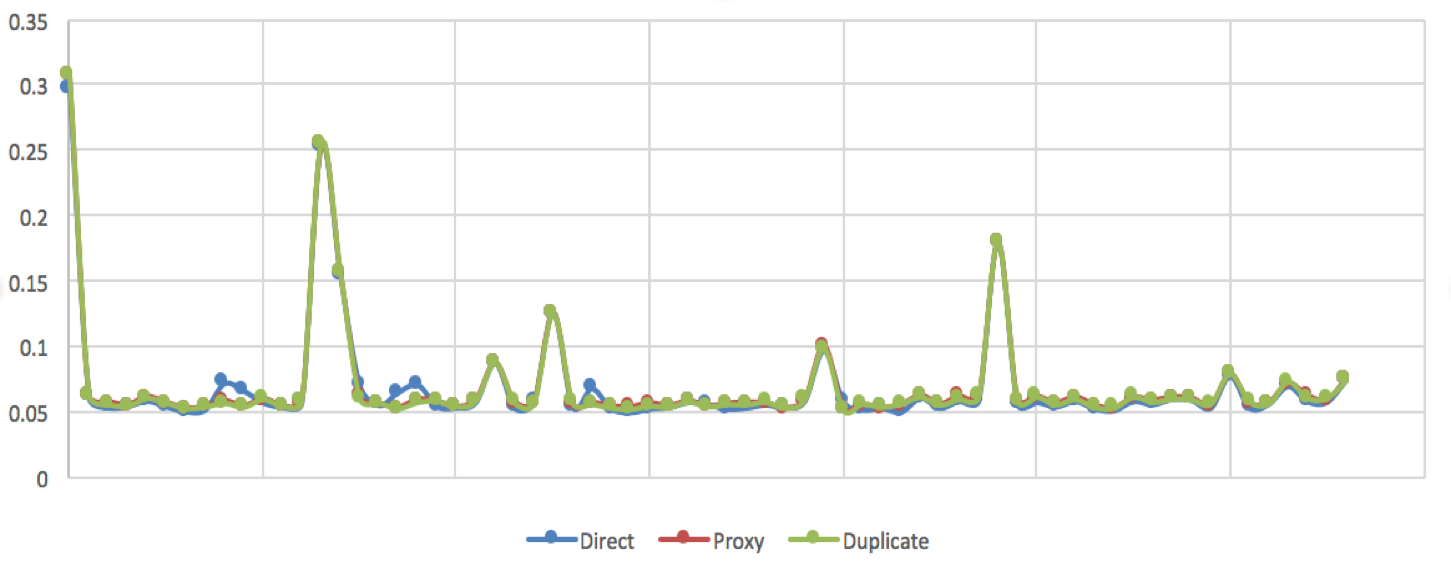
\includegraphics[width=0.9\textwidth]{parikshan/figs/wikipedia_graph.png}
		\caption{Latencies in all different modes for wikipedia trace}
		\label{fig:wikipediaGraph}
	\end{center}
\end{figure}

\begin{table}[]
\centering
\begin{tabular}{ccccc}
\hline
\textbf{Direct} & \textbf{Proxy} & \textbf{Duplication} & \textbf{\begin{tabular}[c]{@{}c@{}}Proxy \\ Overhead\end{tabular}} & \textbf{\begin{tabular}[c]{@{}c@{}}Duplication \\ Overhead\end{tabular}} \\ \hline
0.29702582 & 0.306969121 & 0.306230625 & 3.347 & -0.2405 \\
0.061174009 & 0.06154608 & 0.062500115 & 6.08 & 1.55 \\
0.05342713 & 0.056767733 & 0.055644723 & 6.25 & -1.97825 \\
0.054240793 & 0.054382414 & 0.054373268 & 0.261 & -0.0168 \\
 \hline
\end{tabular}
\caption{Snapshot of the first four latencies of GET/POST requests(secondss) from wikipedia, and the overhead of proxy compared to direct mode, and duplication over proxy mode}
\label{tab:wikibench}	
\end{table}


Firstly we re-created a scaled down deployment of ~\emph{Wikipedia}~\cite{wikipedia}, a well known free online open-source encyclopedia. 
The wikipedia database and application called mediawiki~\cite{mediawiki} is an open-source LAMP (Linux, apache, mysql and PHP stack) application and allows developers to create their own wiki websites.
We leverage wikipedia traces and dumps available through the wikibench~\cite{wikibench} database~\footnote{Please note this database dump does not have most of the wiki images so most of the HTTP requests in our traces, which are image specific had to be filtered out. 
Several post requests, which need user log-ins were also filtered out. 
Hence, we looked at only the requests from the traces which were successful based on the data snapshot available} to re-create the wikipedia application and database in one of our containers.
%The original wikibench is a distributed real-world trace replay to look at the performance of a system under test. 
Once the website was created we used a small sample set of wikipedia HTTP requests traces from 2008, and compared the latency of about 500 HTTP requests in three modes of deployment as we have explained before : Native, Proxy and Duplication. 
We then compared the average change in latencies for each requests.

Table~\ref{tab:wikibench} gives a snapshot of 4 such URL's and it's latencies. 
The second last column gives the overhead of proxy compared to direct communication, whereas the second gives the percentage difference between the duplicate mode as compared to proxy mode.
We found that the proxy was generally slower than the direct connection, the slowdown ranged from 1-8\%, more importantly we found that when comparing the latencies in the duplication mode to our proxy mode, the overhead was negligible and in most cases was less that 2\%. 
Accounting for some variance because of caching, we believe the overhead in a realistic system running with a debugging container will have negligible impact to a similar system running with only a proxy. 

\begin{comment}
One of the difficulties in accurately measuring latencies was that since most GIT page fetches were sub-second, database, and webservers caching came into play. 
This meant that in several of our initial runs the latency observed for some of the requests were better with the proxy or duplicator, compared to the native execution.
However after a couple of runs of the entire trace, the latencies observed were consistent.
\end{comment}

Apart from wikipedia traces we also looked into mysql-server. 
\textbf{Mysqlslap} is a diagnostic program designed to emulate client load for a MySQL server, and to report the timing of each stage. 
It works as if multiple clients are accessing the server. The \emph{mysqlslap} tool runs several iterations of the queries over multiple different parallel connections, and gives an average distribution of the response time for running all queries.
The queries and the test database used is a sample employee database initially provided by Siemens Corporate Research. 
The database contains about 300,000 employee records with 2.8 million salary entries. The export data is 167 MB, which is not huge, but heavy enough to be non-trivial for testing.

We used 5 sample queries, which create 20 concurrent connections, and iterate each of the queries from each of the concurrent threads in 10 iterations.
The \emph{mysqlslap} reports the average number of seconds to run all queries. As is shown below in table~\ref{tab:mysqlslap}, the average amount of time to run all the queries in each of the three modes was found to have minimal difference between the proxy and the duplication modes.

\begin{table*}
	\centering
\begin{center}
	\begin{tabular}{l c}
	\toprule
	\textbf{Modes} & \textbf{mysqlslap}\\
	\midrule
	\textbf{Direct} & 8.220s \\
	\textbf{Proxy} & 8.230s \\
	\textbf{Duplication} & 8.232s \\
	\bottomrule
	\end{tabular}
\end{center}
\caption{Average time to finish \emph{mysqlslap} queries on a sample database}
\label{tab:mysqlslap}
\end{table*}   

\begin{comment}
\noindent \textbf{\underline{Throughput}}\\ 
To check the impact on application throughput, we looked at \emph{httperf}~\cite{httperf},  	
\end{comment}

\begin{tcolorbox}[breakable, enhanced]
	To answer \textbf{RQ3}, we first separated the overhead comparisons between that due to duplication, and that due to an extra-hop because of a proxy. We were able to verify that the performance in terms of both latency and throughput of the duplicator when ~\textbf{compared to a similar system with only a proxy is nearly the same (\textless 2\%)}. The overhead in terms of latency of the proxy vs native communication on was less than 8\% depending on the size of the request and the request processing time in the server. We also verified that ~\textbf{slowdown in the debug container does not have any impact on production service}. 
\end{tcolorbox}